\documentclass{article}
    \usepackage{url}
    \usepackage[margin=0.8in]{geometry}
    \usepackage{cite}    
    \usepackage{amssymb}
    \usepackage{enumerate}
    \usepackage{enumitem}
    \usepackage{graphicx}
    \usepackage{xcolor}
    \usepackage{pdfpages}
    \usepackage{hyperref}
    \usepackage{listings}
    \usepackage{fancybox}
    \usepackage{lstautogobble}
    \usepackage{titling}
    \usepackage{pdflscape}
    \usepackage{afterpage}
    \usepackage[nottoc,notlot,notlof]{tocbibind}
    \renewcommand\maketitlehooka{\null\mbox{}\vfill}
    \renewcommand\maketitlehookd{\vfill\null}

    \newcommand\arduinobackgroundimage{
        \put(-5,0){
        \parbox[b][\paperheight]{\paperwidth}{
        \vfill
        \centering
        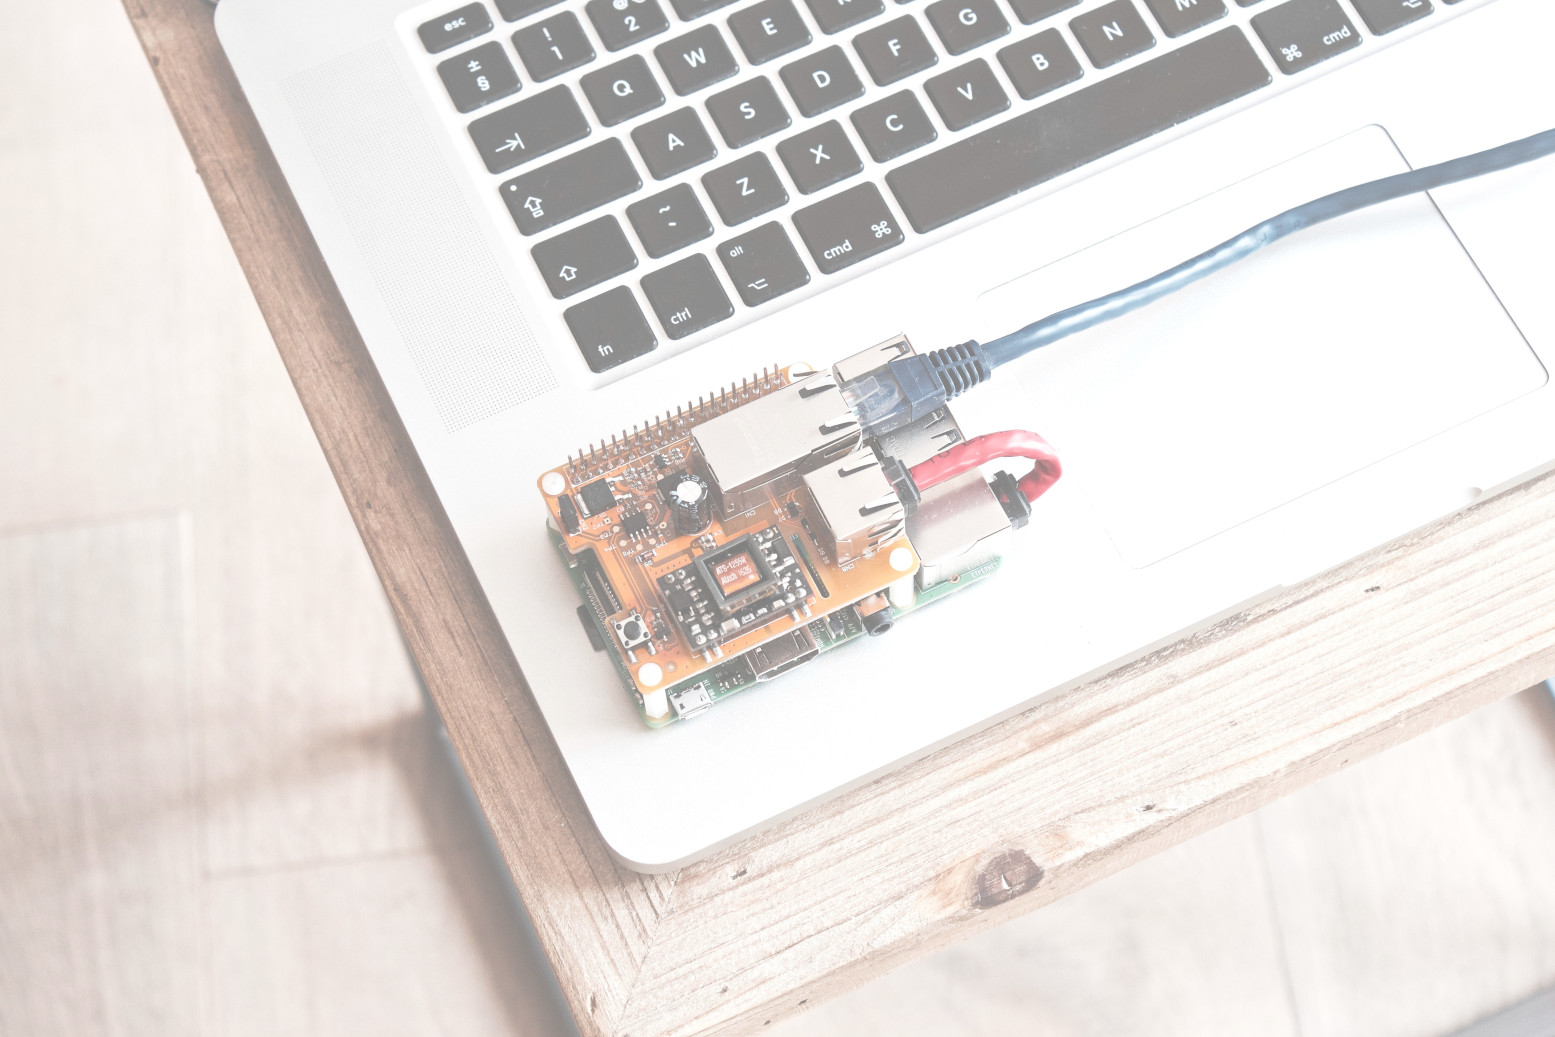
\includegraphics[height=\paperheight]{Images/Arduino.jpg}
        \vfill
    }}}

    \newcommand\usbdocumentbackgroundimage{
        \put(-5,0){
        \parbox[b][\paperheight]{\paperwidth+5px}{
        \vfill
        \centering
        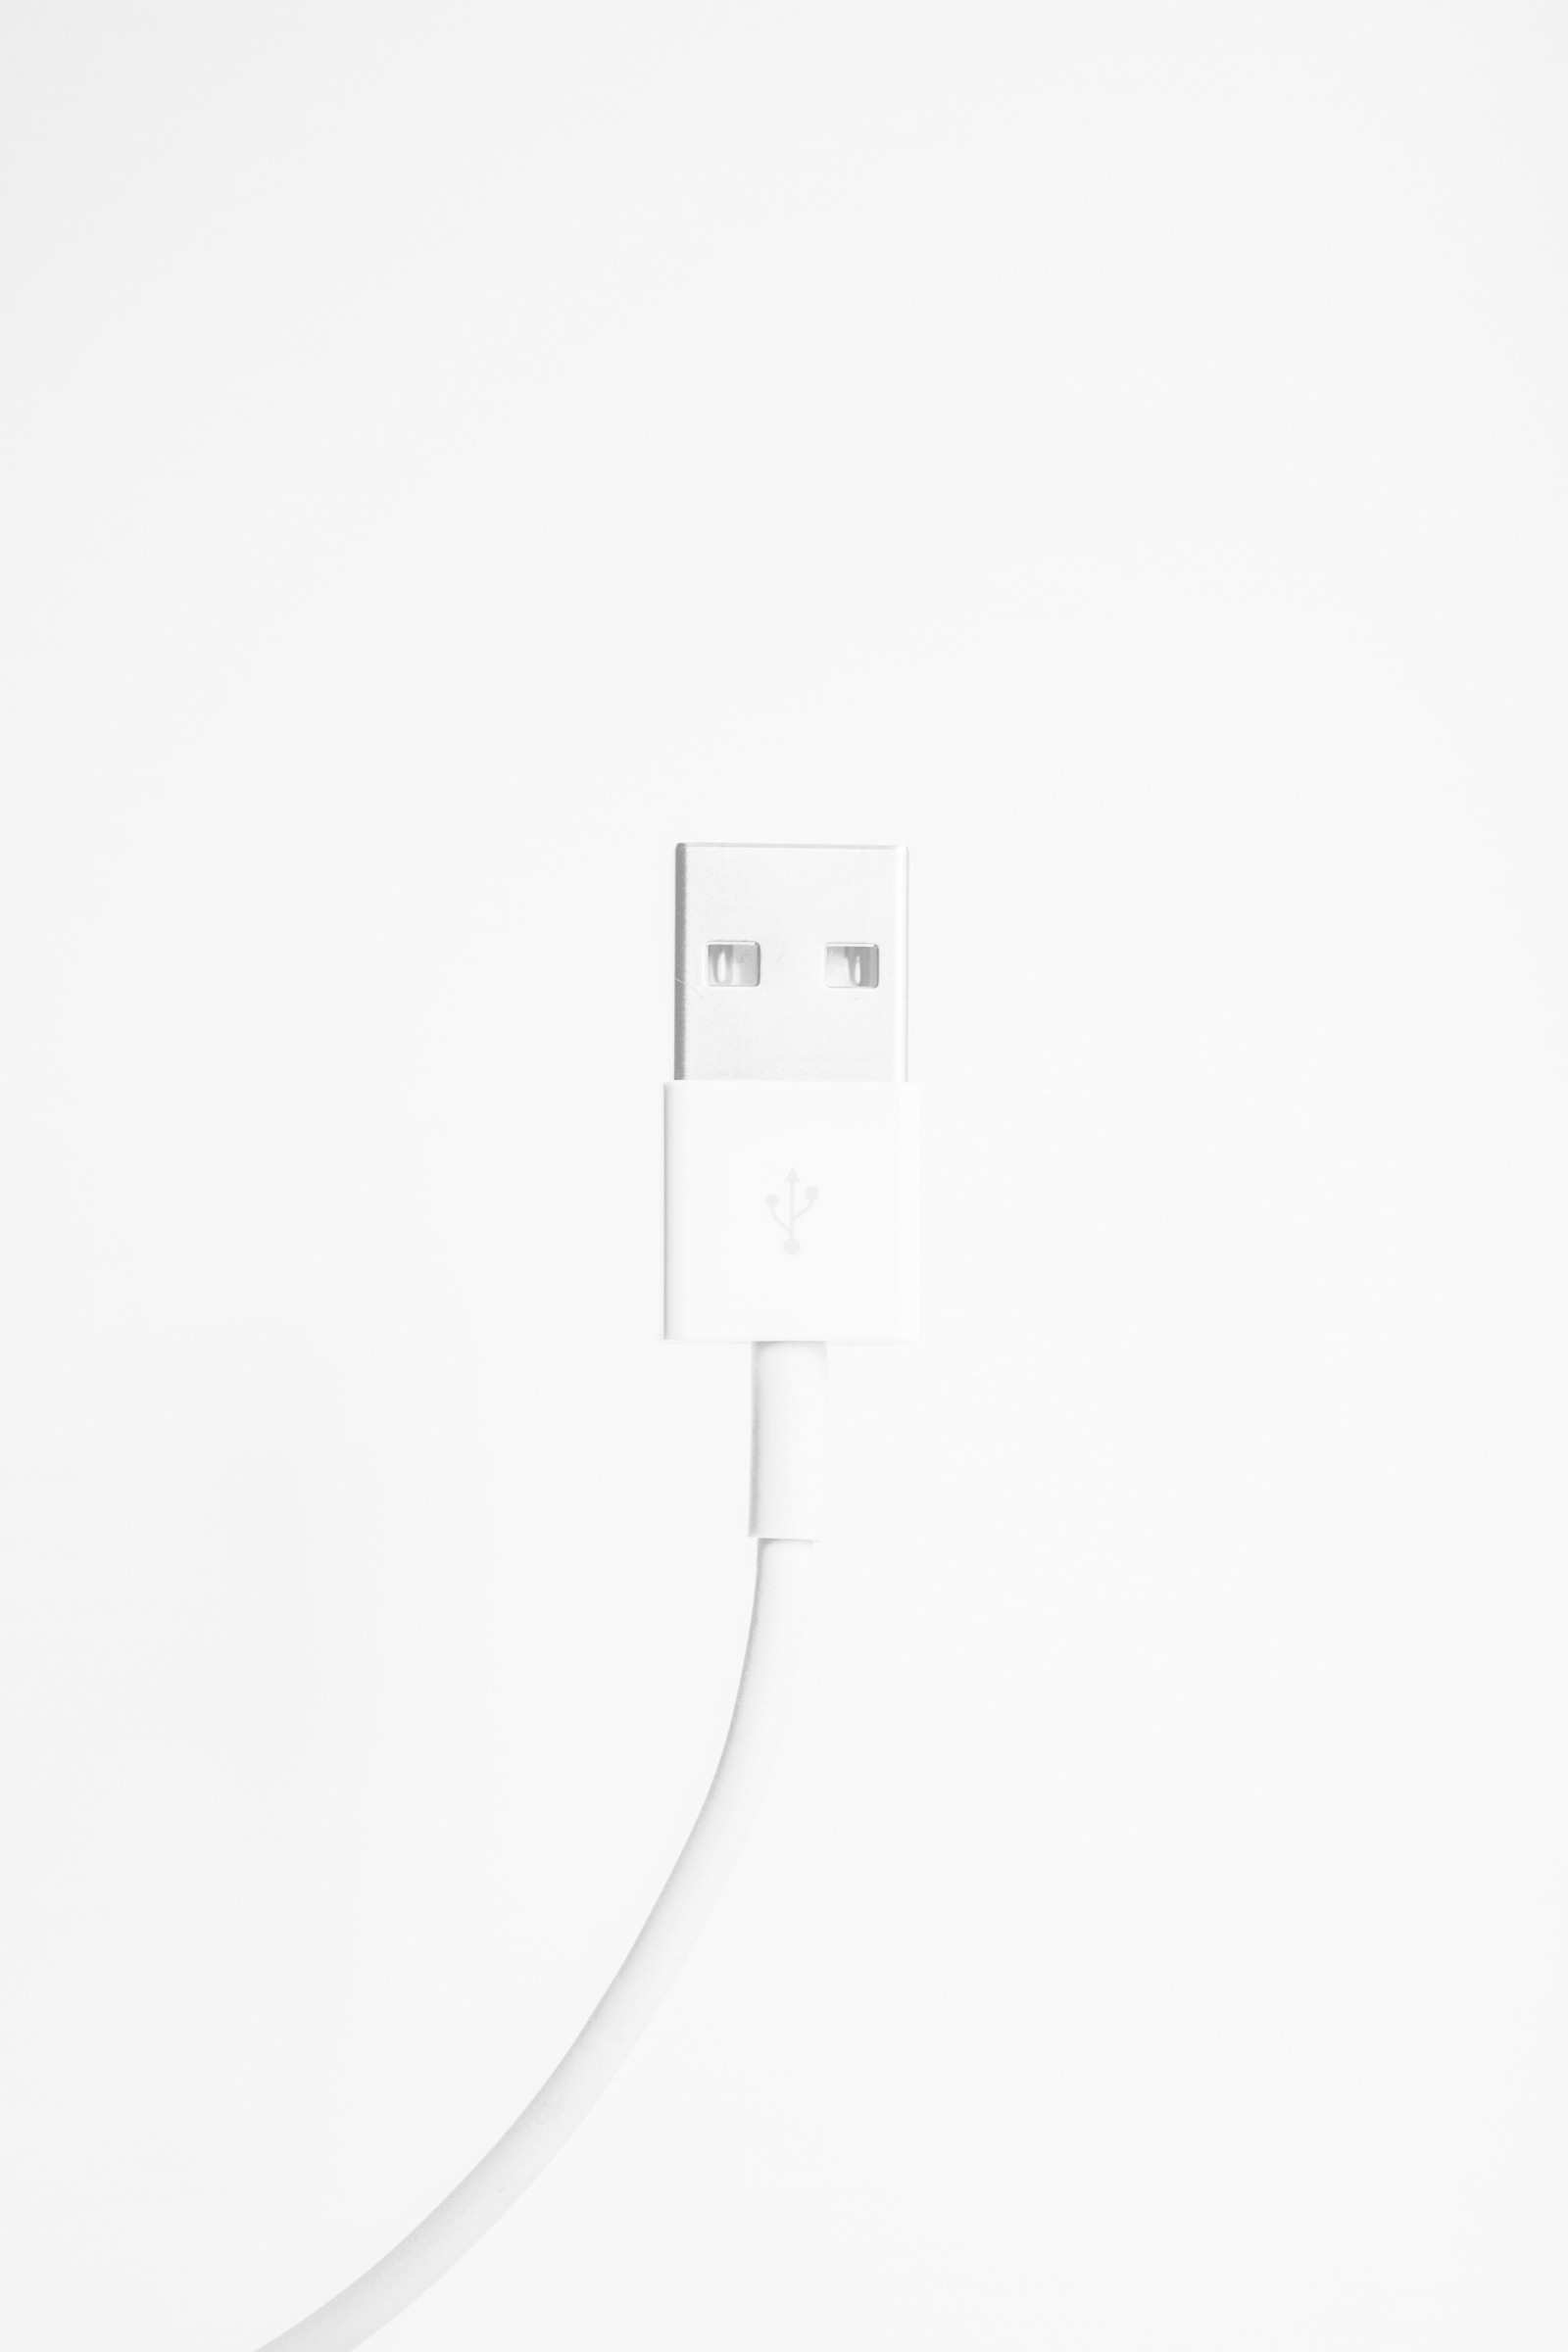
\includegraphics[width=\paperwidth]{Images/USB.jpg}
        \vfill
    }}}

    \newcommand\whitebackgroundimage{
        \put(-5,0){
        \parbox[b][\paperheight]{\paperwidth}{
        \vfill
        \centering
        
\includegraphics[width=\paperwidth]{Images/White.jpg}
        \vfill
    }}}

    \graphicspath{ {Images/} }

    \title{\textbf{INFT3970 Major Project Scope Document \protect\\
    Distributed Monitoring System using Embedded Devices}}
    \author{
        Jay Rovacsek
        \texttt{c3146220@uon.edu.au}\\
        Dean Morton
        \texttt{c3252227@uon.edu.au}\\
        Josh Brown
        \texttt{c3283797@uon.edu.au}\\
        Jacob Litherland
        \texttt{c3263482@uon.edu.au}\\
        Lee Marron
        \texttt{c3263482@uon.edu.au}\\
        Edward Lonsdale
        \texttt{c3252144@uon.edu.au}
    }
    \date{\today}
    \hypersetup{
    colorlinks=true,
    linkcolor=black,
    filecolor=magenta,      
    urlcolor=blue,
    citecolor=red,
    linktoc=section,
    }
    \pagenumbering{arabic}

    \newlist{legal}{enumerate}{10}
    \setlist[legal]{label*=\arabic*.}

    \begin{document}

    \AddToShipoutPicture{\arduinobackgroundimage}

    \begin{titlingpage}
        \maketitle
    \end{titlingpage}

    \AddToShipoutPicture{\usbdocumentbackgroundimage}

    \tableofcontents
    
    \newpage

    \AddToShipoutPicture{\whitebackgroundimage}

    \section*{Executive Summary}
    \vspace{10mm}
        \subsection{Background}
            Riding the wave of "IoT Revolution" \cite{Forbes}, this project will develop
            a low cost, easily deployable IoT product in any setting.
            \\
            IoT or \textit{The Internet of Things} has proven to be an explosive trend within
            the consumer electronics markets. Never before have such small versatile devices been
            available for general consumption, leading to an estimated combined business and
            consumer spending value in excess of \$6 \textit{trillion} dollars globally in 2018\cite{Forbes}.
            \par\noindent
            For the vast majority of consumers, both corporate and end-customer \cite{Mckinsey}, a large 
            movement toward both minimisation of waste and optimisation of spending is occuring
            on a global scale in the developed world, with the developing world rapidly following 
            this trend also\cite{SunNews}.
            \\
            Citing this movement, it would only be logical to create a simple to use set of devices 
            that allow for the monitoring and therefore optimisation of such measurables.
        \vspace{10mm}
        \subsection{Overview and Purpose}
            The concept of this project is to create a distributed system in which small 
            devices are used to monitor, log and analyse a number of select metrics from a 
            multitude of potential data points.
            \par\noindent
            The purpose of the project is to deliver a viable product that could be replicated
            for a reasonable price for both end-user and business alike. We believe the market to
            be on a precipice of further explosive growth, with the consumer market partially
            realised, but far from tapped by curent offerings.
            \par\noindent
            In this document we intend 
            \subsubsection{Metrics}
                The metrics measured included will be: 
                \begin{itemize}
                    \item Temperature
                    \item Humidity
                    \item Motion
                \end{itemize}
                We anticipate further development on the project to be viable post submission date,
                however realise the limitations of the current timeframe.
                \par
                Metrics measured would be viewable on a users dashboard, with data being able to be
                scoped to multiple filter requirements such as time, select edge cases or specific 
                locations.
                \\
                The end-goal being an ability for users to better determine inefficient or bad decisions
                they may make unwittingly in regards to home or business heating, coupled with the 
                impact of room utilisation.

    \newpage

    \section{Project Objectives}
        Within the timeframe still available to this project, we aim to develop and deploy a number of 
        IoT devices\cite{ESP8266} to a home enviroment or two and to track heat, humidity and motion of the
        dwelling to better understand the potential correlations of room use, heating and potential 
        inefficiencies created in areas such as 'High Traffic' spots (Loungerooms and Hallways)
        \\
        Optimally we ain to couple this with a mapping of the dwelling, allowing a more intuitive expression 
        of the data collected.
        \par
        We intend on using student subscriptions to leverage Azure for both website hosting and databasing 
        coupled with a small budget of roughly \$100-\$200 to purchase all required equipment which currently
        is expected to be:
        \begin{itemize}
            \item Arduino UNO3 Microcontroller
            \item ESP8266 boards
            \item DHT11 Temperature and Humidity sensors\cite{DHT11}
            \item XC-4444 PIR Motion sensors\cite{XC-4444}
            \item Various required breadboards / generic electronics items
        \end{itemize}

        \vspace{10mm}

        \subsection{Deliverables}
            Included deliverables for the project will include a large span of items crossing a number
            of percieved IT-sub-disciplines:
            \begin{itemize}
                \item Raw data be stored in an online database including:
                \begin{itemize}
                    \item Temperature
                    \item Humidity
                    \item Motion
                    \item Associated timestamps for datapoints
                    \item User information including:
                    \begin{itemize}
                        \item Name
                        \item Address
                        \item Postcode
                    \end{itemize}
                \end{itemize}
            \end{itemize}

            The user interface will be developed to allow the users to access their stored
            infomation and optionally remove sections of data. Each user will be able to customise 
            their own homepage in order to display to their needs. The user interface will deliever:
            \begin{itemize}
                \item Login page
                \item Registration
                \item Home Page (Where all data is displayed)
                \item Graphs based on the user's data
                \item Analytic results
                \item Suggestions
                \item Logout
            \end{itemize}
            \newpage

        \subsection{Milestones}
            Major milestones for the project include are split into a number of 
            concurrently developed sub-sections:
            \\
            \begin{legal}
                \item Sensors:
                \begin{legal}
                    \item Sensor proof of concept implementation (serial to USB)
                    \item Testing of POC
                    \item Sensor and Wifi Implementation
                    \item Testing of Sensor and Wifi implementation
                    \item Sensor to API communication including:
                    \begin{legal}
                        \item Implementation and testing of Temperature logging
                        \item Implementation and testing of Humidity logging
                        \item Implementation and testing of Motion logging
                        \item Testing of Sensor to API communication
                    \end{legal}
                \end{legal}
                \item Database:
                \begin{legal}
                    \item Database Pilot
                    \item Review and Testing of Database
                    \item Optimisation of datatypes used in each table
                    \item Implementation of indexing and other optimisations to avoid big O issues.
                    \item Final database implementation.
                \end{legal}
                \item Backend:
                \begin{legal}
                    \item Decision of framework to be used
                    \item Initial POC on framework
                    \item Feature implementations: 
                    \begin{legal}
                        \item Implementation of PING GET endpoint to avoid sending of data unnecessarily
                        \item Implementation and testing of POST endpoints:
                        \begin{legal}
                            \item Temperature
                            \item Humidity
                            \item Motion
                        \end{legal}
                        \item Implementation and testing of application helpers to aid front-end data sourcing
                    \end{legal}
                    \item Refactor existing code
                    \begin{legal}
                        \item Peer review of code, implementation of required changes
                    \end{legal}
                \end{legal}
                \item Front End:
                \begin{legal}
                    \item Initial implementation of POC dashboard
                    \item Initial POC of authentication using a login page
                    \item Review of code by peers
                    \item Migrate dashboard behind successful login page
                    \item Improvements and refactoring of dashboarding code
                    \item Review and refactor to suit all devices commonly used to browse websites.
                    \item Implement required bootstrap/css framework to handle display of data.
                    \item Final peer review and refactor
                \end{legal}
                \newpage
                \item Documentation
                \begin{legal}
                    \item Generate POC documentation from project
                    \item Generate scope document
                    \item Comment code extensively for readability
                    \item Document APIs
                    \item Document database design, with considerations of optimisation and required modifications
                    \item Generate user guide for final product
                    \item Generate final report
                \end{legal}
            \end{legal}
        \newpage
    
    \section{Technical Requirements}
        Requirements for raw data be stored in an online database are only access
        for the development resources to be able to access any suitable cloud account, 
        self-host on a local machine or debug required functions in the application with 
        localised datageneration via ajax queries of similar methods.
        \\
        Pages for the site itself will require a suitable host either cloud or local which
        supports .NETcore 2.0\cite{DotNetCore2} and suitable network access to reach a
        required TSQL\cite{TSQL} database hosted by the team.
        \vspace{5mm}

        Functioning network connectivity, all of the sensors will be connected to a local network which will 
        then send all the data to the API. Having the local network is vital part to the success of the system 
        as the sensors will not be able to communicate with the database.
        \par
        Meet system requirements to run the users preference of web browser, the user will have to login into 
        the system through a local web browser to view their sensor information on their network.
        \vspace{5mm}

        Azure to run the Database and website hosting. The database will be used to store all the data that is 
        sent from the sensors. The uptime of the database the web application is vital to the user experience 
        and the success of the project. Azure provides this security with 99.95\% uptime \cite{AzureUptime}.
        \par
        SQL management studio to manage the database. Azure is using TSQL which can be managed by SQL management studio 
        on the developers local machine. Visual studio to develop the front and back end of the web application. 
        The development of the web application will be written in visual studio then pushed to azure for final deployment.
        Arduino boards and sensors. ESP8266 boards will be used with a variety of compatible sensor to create a home 
        monitoring system. These sensors include temperature, humidity and motion.\\
        Arduino IDE software for editing/flashing the boards in C/C++

    
        Majority of product/service has the “requirements”\\
        More details than deliverables.

    \section{Limitations}
        It is important to acknowledge the limitations of this project, given that this project is taking place 
        in a compressed format it will primarily be an exploratory exercise in IOT sensor technology and its 
        ability to interface with middleware frontend/backend and an SQL server implementation.
        \par
        In order to managing expectations we are primary focused on heat,humidity and motion, this proof of 
        concept implementation reduces the risk of under delivering on expectations.

        “Limitation” of the project\\
        Managing expectation, not over-promising

        \newpage

    \begin{thebibliography}{9}
        \raggedright
        \bibitem{Forbes}
            \url{https://www.forbes.com/sites/danielnewman/2017/12/19/the-top-8-iot-trends-for-2018/}
        \bibitem{Mckinsey}
            \url{https://www.mckinsey.com/business-functions/digital-mckinsey/our-insights/the-internet-of-things-the-value-of-digitizing-the-physical-world}
        \bibitem{SunNews}
            \url{http://sunnewsonline.com/china-is-worlds-largest-renewable-energy-producer-consumer/}
        \bibitem{ESP8266}
            \url{http://esp8266.net/}
        \bibitem{XC-4444}
            \url{https://www.jaycar.com.au/medias/sys_master/images/9105858396190/XC4444-dataSheetMain.pdf}
        \bibitem{DHT11}
            \url{https://www.jaycar.com.au/medias/sys_master/images/9091897786398/XC4520-dataSheetMain.zip}
        \bibitem{DotNetCore2}
            \url{https://www.microsoft.com/net/download}
        \bibitem{TSQL}
            \url{https://docs.microsoft.com/en-us/sql/t-sql/language-reference?view=sql-server-2017}
        \bibitem{AzureUptime}
            \url{https://azure.microsoft.com/en-au/support/legal/sla/app-service/v1_4/}
    \end{thebibliography}

    \end{document}
